\chapter{Cryptographic Techniques}
\cite{02_basic_crypto}.
Cryptography is the practice of securing communication and data by transforming it into a format that is unreadable to unauthorized users. It uses mathematical algorithms to encrypt (scramble) and decrypt (unscramble) information, ensuring confidentiality, integrity, authentication, and non-repudiation in digital communications.

The message in its original, unencrypted form is called plaintext (or cleartext), referred to as P. On the other hand, the message after being encrypted is called ciphertext, referred to as C. 

\section{Kerchoffs' Principle}
\begin{quotation}
    If the keys are kept secret, managed securely, and are of sufficient length, the system remains secure even if the encryption and decryption algorithms are publicly known. This is because, without access to the keys, an attacker cannot decrypt the data. In fact, making the algorithms public allows the cryptographic community to rigorously test and analyze them for potential weaknesses, improving the overall security of the system.
\end{quotation}

\section{Symmetric Cryptography}
\begin{center}
    Only one key, shared between the sender and the receiver, is used for both encryption and decryption. 
\end{center}

\textbf{Encrypt Equation}
\begin{equation*}
    \begin{aligned}
        C &= \text{enc}(K, P) \\
          &= \{ P \}_K
    \end{aligned}
\end{equation*}

\hfill

\textbf{Decrypt Equation}
\begin{equation*}
    \begin{aligned}
        P &= \text{dec}(K, C) \\
          &= \text{enc}^{-1}(K, C)
    \end{aligned}
\end{equation*}
\begin{figure}[H]
    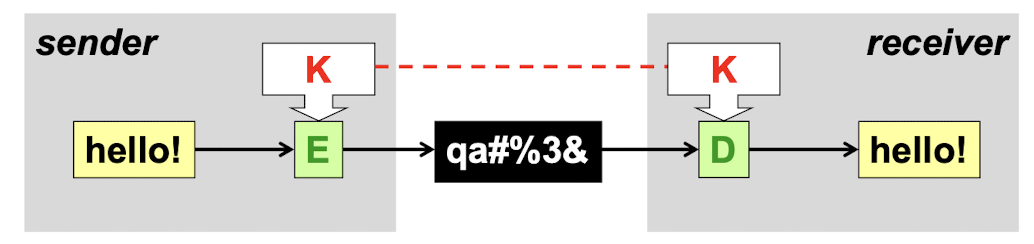
\includegraphics[width=\linewidth]{Images/Cryptography/symmCrypto.png}
    \caption{Example of symmetric encryption}
\end{figure}

\section{Symmetric Block Encryption Algorithms}
Block encryption refers to ciphers that process fixed-size blocks of data (e.g., 128 bits) at a time.

\begin{figure}[H]
    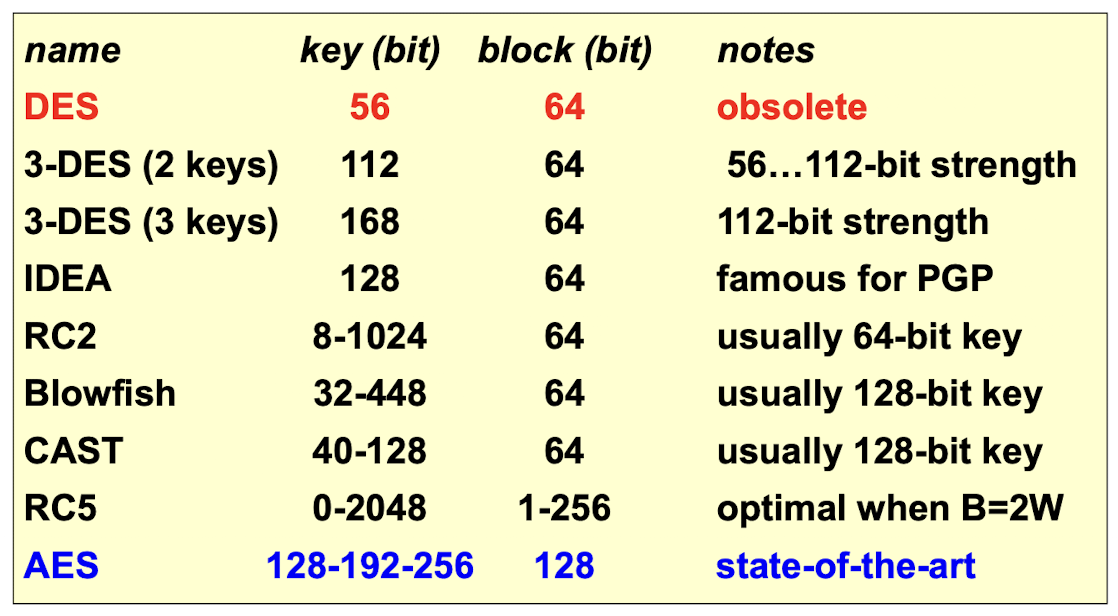
\includegraphics[width=\linewidth]{Images/Cryptography/blockSymm.png}
    \caption{Famous Symmetric Block Encryption Algorithms}
\end{figure}


\subsection{DES}
\begin{center}
    (Data Encryption Standard - Obsolete because of short key length)
\end{center}
Is a symmetric-key block cipher that was widely used for data encryption in the past. It was developed in the 1970s by IBM.

The key features are:
\begin{itemize}
    \item Block cipher: DES operates on 64-bit (8 bytes) blocks of data, meaning it encrypts 64 bits of plaintext at a time.
    \item Key length: DES uses a 56-bit (7 bytes) key.
    \item Efficient in hardware: Requires only XOR, shift and permutation.
\end{itemize}

\subsection{Triple DES}
\begin{center}
    (3DES or TDES)
\end{center}

Is a symmetric-key block cipher that was developed to enhance the security of the original DES.

The key features are:
\begin{itemize}
    \item Block cipher: like DES (8 bytes).
    \item Key Length: 3DES can use either:
    \begin{itemize}
        \item \textbf{Two keys} (2-key 3DES): The first and third keys are the same, resulting in a 112-bit effective key length.
        \item \textbf{Three keys} (3-key 3DES): All three keys are distinct, resulting in a 168-bit effective key length.
    \end{itemize}
    \item Triple encryption: 3DES applies the DES algorithm three times to each data block, using either two (2-key 3DES) or three (3-key 3DES) distinct keys.
    \item Is typically applied in the Encrypt-Decrypt-Encrypt (EDE) mode to achieve compatibility with DES when.
\end{itemize}

\subsubsection{EDE Mode}
In this mode, the data is first encrypted using the first key, then decrypted using the second key, and finally encrypted again using the third key (if a third key is present). This sequence of operations helps mitigate the vulnerabilities of DES by applying encryption multiple times.

\begin{tcolorbox}[colback=blue!10!white, colframe=blue!50!white, title=Meet-in-the-Middle attack]
    Double application of encryption algorithms is subject to a known plaintext attack named meet-in-the-middle, which allows decrypting data with at most $2^{N+1}$ attempts (the key is N-bit long).
    For more details, refer to Appendix A.
\end{tcolorbox}

\section{Application of Block Algorithms}
We should answer a question:
\begin{tcolorbox}[colframe=lightblue]
    \begin{center}
        \textit{Is the size of the encrypted data smaller or larger than \newline the algorithm’s block size?}
    \end{center}
\end{tcolorbox}
    

If the answer is:
\begin{itemize}
    \item Size of the encrypted data > algorithm's block size: Use Electronic Code Book (ECB) or Cipher Block Chaining (CBC).
    \item Otherwise: Padding, Cipher FeedBack (CFB), Output FeedBack (OFB) or Counter Mode (CTR).
\end{itemize}

\subsection{Electronic Code Book}
\begin{center}
    (ECB)
\end{center}

Simple mode of operation for block ciphers. In this mode, the plaintext is divided into fixed-size blocks, and each block is encrypted independently using the same key.

\begin{multicols}{2}
    \begin{equation*}
        \boxed{C_i = enc \ (K, P_i)}
    \end{equation*}
    \begin{figure}[H]
        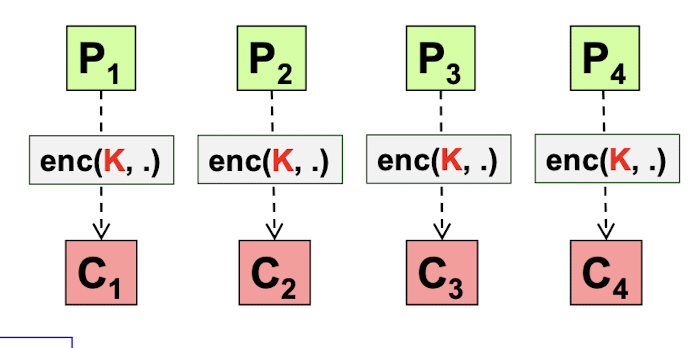
\includegraphics[width=\linewidth]{Images/Cryptography/ECBEncrypt.png}
        \caption{ECB encrypting.}
    \end{figure}
    \columnbreak
    \begin{equation*}
        \boxed{P_j = \text{enc}^{-1}(K, C_j)}
    \end{equation*}
    \begin{figure}[H]
        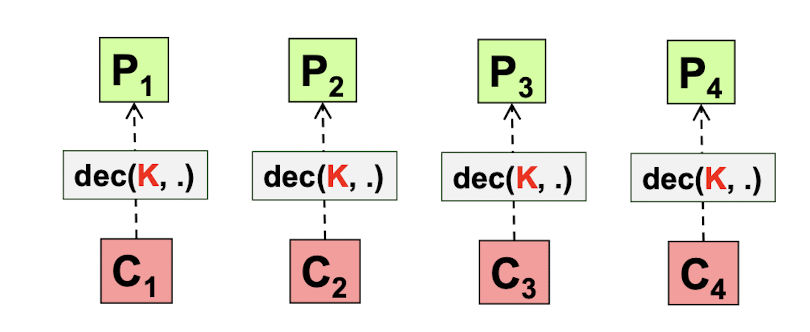
\includegraphics[width=\linewidth]{Images/Cryptography/ECBDecrypt.png}
        \caption{ECB decrypting.}
    \end{figure}
\end{multicols}

Key features:
\begin{itemize}
    \item Should not be used for long messages because swapping two blocks of ciphertext goes undetected, and identical plaintext blocks generate identical ciphertext blocks, making it vulnerable to known-plaintext attacks.
    \item The plaintext is divided into blocks of equal size (typically 64 or 128 bits, depending on the cipher)
    \item Each block is encrypted separately with the block cipher using the same key.
    \item The encrypted blocks are concatenated to produce the ciphertext.
    \item Identical plaintext blocks produce identical ciphertext blocks, which can lead to patterns in the ciphertext that may be exploited in cryptanalysis.
    \item If there is an error in one ciphertext block  $C_j$ , only the corresponding plaintext block  $P_j$  will be affected during decryption.
\end{itemize}

\clearpage
\subsection{Cipher Block Chaining}

\begin{center}
    (CBC)
\end{center}
Mode of operation for block ciphers that provides better security than Electronic Codebook (ECB). It involves chaining the encryption of each block with the previous block’s ciphertext, which helps obscure patterns in the ciphertext.


\begin{multicols}{2}
    \begin{equation*}
        \boxed{C_i = enc \ (K, P_i \oplus C_i-1)}
    \end{equation*}
    \begin{figure}[H]
        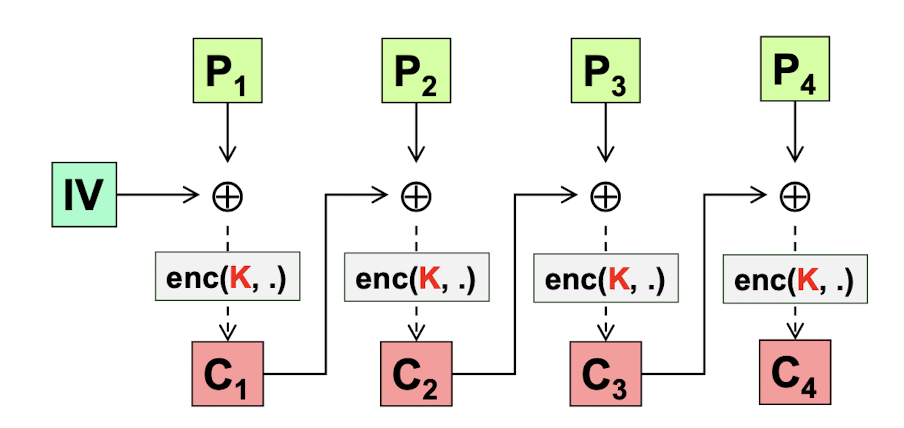
\includegraphics[width=\linewidth]{Images/Cryptography/CBCEncrypt.png}
        \caption{ECB encrypting.}
    \end{figure}
    \columnbreak
    \begin{equation*}
        \boxed{P_j = \text{enc}^{-1}(K, C_j) \oplus C_{j-1}}
    \end{equation*}
    \begin{figure}[H]
        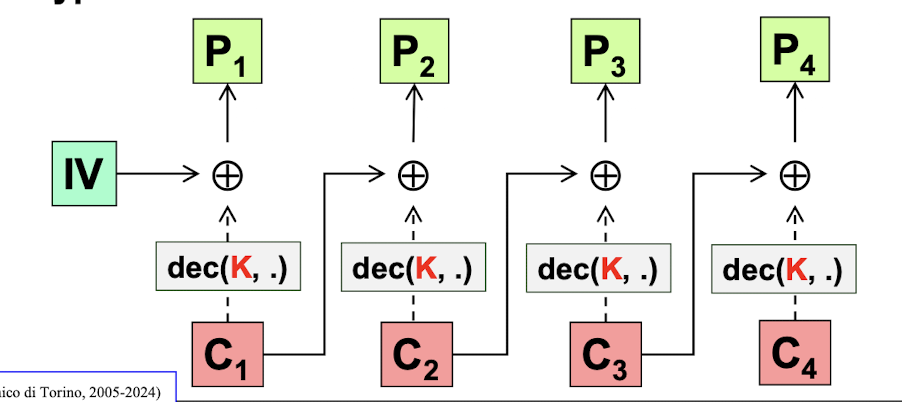
\includegraphics[width=\linewidth]{Images/Cryptography/CBCDecrypt.png}
        \caption{ECB decrypting.}
    \end{figure}
\end{multicols}

Key features:
\begin{itemize}
    \item Requires an Initialization Vector (IV=$C_0$).
    \item XOR between ciphertexts and plaintexts.
    \item If there is an error in a ciphertext block $C_j$ it will affect the decryption of two blocks of plaintext:
    \begin{itemize}
        \item The current block $P_j$ will be corrupted because the error will be decrypted into some incorrect plaintext. 
        \item The next block  $P_{j+1}$  will also be corrupted because the error will propagate into the XOR operation with the next ciphertext block  $C_{j+1}$.
    \end{itemize} 
\end{itemize}

\subsection{Padding}
\begin{center}
    (aligning, filling)
\end{center}

Padding modes are used in block cipher encryption schemes to handle plaintext that is not an exact multiple of the block size. Since block ciphers operate on fixed-size blocks, any plaintext that does not fit into the required block size needs to be padded.
\begin{figure}[H]
    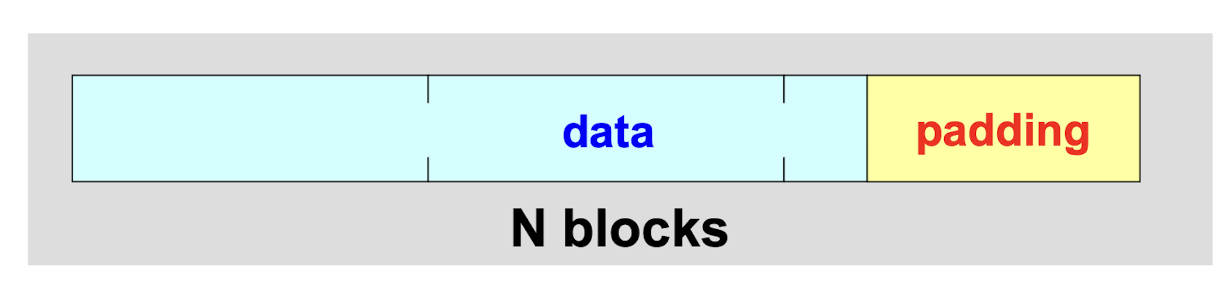
\includegraphics[width=\linewidth]{Images/Cryptography/padding.png}
    \caption{Padding Mode}
    
\end{figure}

\subsubsection{Padding Techniques}
\begin{itemize}
    \item If the length is known, add null bytes as padding.
    \item Original DES Padding: bit pattern that started with a 1 bit, followed by many 0 bits.
\end{itemize}

